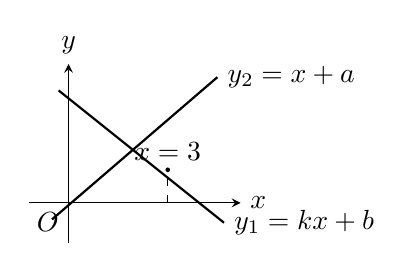
\begin{tikzpicture}[scale=0.42,>=stealth]
  \draw[->] (-1.2,0)--(5.2,0) node[right] {$x$};
  \draw[->] (0,-1.2)--(0,4.2) node[above] {$y$};
  \draw[thick] (-0.3,3.4)--(4.7,-0.6) node[right] {$y_1=kx+b$};
  \draw[thick] (-0.5,-0.5)--(4.5,3.8) node[right] {$y_2=x+a$};
  \fill (3,1.0) circle (2pt) node[above] {$x=3$};
  \draw[dashed] (3,0)--(3,1.0);
  \node[below left] at (0,0) {$O$};
\end{tikzpicture}
